\documentclass[aspectratio=169]{beamer}

\graphicspath{{figures/}{../figures/}}

% Кириллица: pdfLaTeX -- через T2A, XeLaTeX/LuaLaTeX -- через системные шрифты.
\usepackage{iftex}
\ifPDFTeX
  \usepackage[T2A]{fontenc}
  \usepackage[utf8]{inputenc}
\else
  \usepackage{fontspec}
  \setsansfont{Arial}
\fi
\usepackage[english,russian]{babel}
\usepackage{amssymb,amsmath}
\usepackage{booktabs}

\usecolortheme{beaver}
\usefonttheme[onlymath]{serif}
\setbeamertemplate{navigation symbols}{}
\setbeamertemplate{footline}{}
\setbeamersize{text margin left=0.4cm,text margin right=0.4cm}
\setbeamerfont{frametitle}{size=\normalsize}

\title{CRISP: самоигра Challenger--Reasoner на основе корпуса документов}
\author{Роман Акрамов \quad Научный руководитель: Р.\,В.~Ищенко}
\date{}

\begin{document}

\begin{frame}{CRISP: GRPO на сгенерированных вопросах --- на уровне публичных математических датасетов}
\vspace{-12pt}
\centering
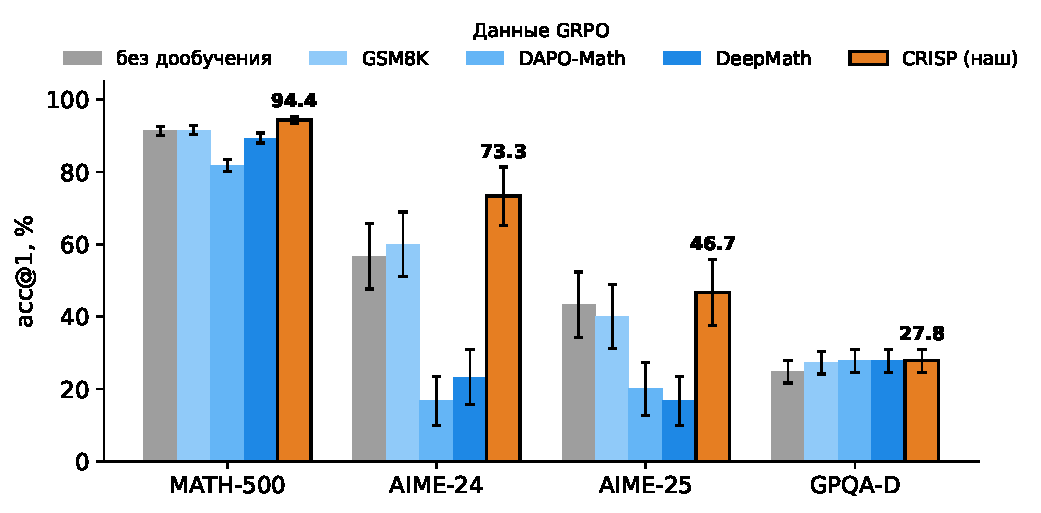
\includegraphics[width=0.97\textwidth]{oslide_main.pdf}

\vspace{-2pt}
\begin{columns}[T]
\begin{column}{0.49\textwidth}
\tiny
\textbf{Что сравниваем.} Одна модель Qwen3-14B (Base и Instruct), один рецепт GRPO; меняются только обучающие данные. Вопросы CRISP получены без разметки: 766 PDF $\to$ OCR $\to$ корпус $\to$ самоигра Challenger (видит документ) / Reasoner (не видит) $\to$ отбор LLM-судьёй.

\textbf{Обозначения.} acc@1 --- доля верных ответов, среднее по 3 сэмплам ($T{=}0.6$); усы --- $\pm1$ std биномиального шума (в AIME 30 задач).
\end{column}
\begin{column}{0.49\textwidth}
\tiny
\textbf{Среднее acc@1 по 9 бенчмаркам, \%} (без дообучения / GSM8K / DAPO-Math / DeepMath / \textbf{CRISP}):\\
Base: 58.9 / 65.7 / 63.8 / 64.1 / \textbf{63.0}; \quad Instruct: 75.2 / 75.2 / 65.7 / 67.9 / \textbf{77.3}.

\textbf{Итог.} На Base вопросы CRISP дают прирост того же порядка, что и публичные датасеты ($+4.1$ против $+4.9$...$+6.8$ п.п.). На Instruct не ухудшают модель ($+2.1$), тогда как DAPO-Math и DeepMath снижают среднее на 7--10 п.п.
\end{column}
\end{columns}
\end{frame}

\end{document}
